% ch10a Bosonization, part a (书页 146-161 / 分册p001-016；10.3节末尾（分册p17顶部）文字见 ch10b 顶部 %--TAIL--)
% 第10章 Bosonization
\chapter{玻色化}

让我们细致考察在发生等离体振荡（plasma oscillations）的极限下，电子密度的傅里叶分量的有效运动方程。我们在上一章中证明，在 $\omega_{\mathrm{p}}^{2}\gg k^{2}v_{\mathrm{F}}^{2}$ 的极限下，各傅里叶分量服从运动方程
\begin{equation*}
\ddot{\rho}_{k}+\omega_{\mathrm{p}}^{2}\rho_{k}=0,
\tag{10.1}
\end{equation*}
即谐振子的运动方程。然而，谐激发服从玻色统计。这暗示等离体振荡在某种程度上代表着相互作用电子气的玻色型激发。等价地，可以把等离体振荡看作气体中电子的谐激发。这种局面会对电子气产生深远的后果；这一点最初由朝永（Tomonaga，T1950）指出，他给出了在稠密费米体系中构造声波谱的明确方案。三年后，玻姆（Bohm）和 Pines（BP1953）证明了声波（玻色型）谱与无规相位近似（RPA）之间存在自然的联系。从那时起，稠密费米体系中的长波激发与玻色子集合之间的等价性，在固体物理以及相对论性场论中都被证明具有根本性的重要意义。本章中，我们聚焦于这样一个问题：一维中服从标准反对易关系的相互作用电子集合，如何能用一组等价的玻色模式来描述。为一个费米子集合构造这样一种玻色场论的问题，称为玻色化（bosonization）。沿着这一思路，我们将先对一维哈伯德（Hubbard，H1964）模型的色散关系作线性化，并由此得到卢廷格液体（Luttinger liquid，L1960），然后再用玻色化求解它。只要这类体系由短程库仑相互作用主导，卢廷格液体就构成分析一维相互作用电子性质的一般基础。我们将导出卢廷格液体理论最引人注目的预言之一——自旋–电荷分离（spin–charge separation），即电子的自旋自由度与电荷自由度解耦并以不同的速度传播。

\section{卢廷格液体}

在引入卢廷格模型（L1960）之前，我们先回顾一下非相互作用电子激发谱的形式。一维晶格上的电子可以由如下哈密顿量给出的紧束缚模型描述：
\begin{equation*}
H_{\mathrm{F}}=-t\sum_{n\sigma}\left[\Psi_{n\sigma}^{\dagger}\Psi_{n+1\sigma}+\mathrm{h.c.}\right]+\mu\sum_{n\sigma}\Psi_{n\sigma}^{\dagger}\Psi_{n\sigma},
\tag{10.2}
\end{equation*}
其中 $t$ 是相邻格点之间的跃迁积分，晶格常数为 $a$。算符 $\Psi_{n\sigma}$ 湮灭格点 $n$ 上一个自旋为 $\sigma$ 的电子，$\mu$ 是有序体系的化学势，而 $\rho_{n\sigma}=\Psi_{n\sigma}^{\dagger}\Psi_{n\sigma}$ 是第 $n$ 个格点上的电子密度。$H_{\mathrm{F}}$ 所描述的模型具有对称能带 $\epsilon_{k}=-2t\cos ka+\mu$。自由空间中的电子具有抛物线型色散 $\epsilon_{k}=\hbar^{2}k^{2}/2m+\mu$。这两条能带均画在图 10.1 中。

\begin{figure}[H]\centering
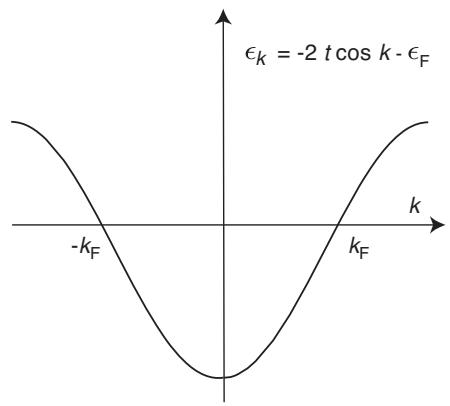
\includegraphics[width=0.42\textwidth]{figs/ch10/fig_10.1_a.jpg}\hfill
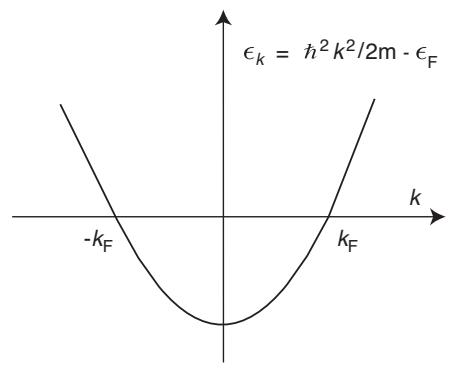
\includegraphics[width=0.42\textwidth]{figs/ch10/fig_10.1_b.jpg}\\[2pt]
{\small\makebox[0.42\textwidth][c]{(a)}\hfill\makebox[0.42\textwidth][c]{(b)}}\\[10pt]
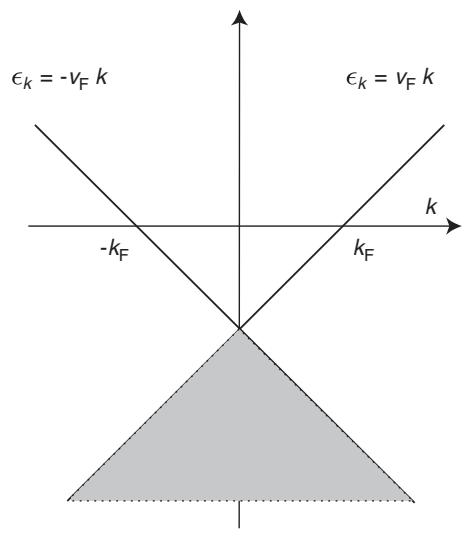
\includegraphics[width=0.42\textwidth]{figs/ch10/fig_10.1_c.jpg}\\[2pt]
{\small (c)}
\caption*{图 10.1\quad (a) 一维非相互作用电子在晶格模型中的能带与 (b) 自由空间模型中的能带（$\epsilon_{\mathrm{F}}=-\mu$）。(c) 费米面附近线性化的能带。阴影区域表示负能量态的填充，即狄拉克海（Dirac sea）。}\label{fig:auto:10.1}
\end{figure}

自由体系的基态中，所有动量 $|k|\leqslant k_{\mathrm{F}}$ 的态都被双重占据（例如 $\mu=0$ 对应 $k_{\mathrm{F}}=\pi/2a$）。无论单粒子态的填充如何，费米面附近的色散关系总可以线性化，得到图 10.1(c) 所示的谱。卢廷格液体模型 $H_{\mathrm{L}}=H_{\mathrm{F}}+H_{U}$ 可以由一维哈伯德模型导出，后者包含一个相互作用项
\begin{equation*}
H_{U}=U\sum_{n}\rho_{n\uparrow}\rho_{n\downarrow},
\tag{10.3}
\end{equation*}
它就是用自旋相反的电子双重占据任一格点所需付出的能量代价，$U$ 是在位（on-site）库仑能。在第 7 章讨论安德森杂质时，我们曾用在位原子轨道定义在位排斥。现在的目标是：在费米点 $\pm k_{\mathrm{F}}$ 附近对单粒子谱取线性近似，把 $H_{\mathrm{L}}$ 改写成等价的玻色描述。

我们现在演示如何把一维费米面的色散关系线性化。形式上，做法是把每个自旋在 $\pm k_{\mathrm{F}}$ 附近的格点振幅写成左移费米场 $\Psi_{n\sigma-}$ 与右移费米场 $\Psi_{n\sigma+}$ 的线性组合
\begin{equation*}
\Psi_{n\sigma}=\mathrm{e}^{\mathrm{i}k_{\mathrm{F}}na}\Psi_{n\sigma+}+\mathrm{e}^{-\mathrm{i}k_{\mathrm{F}}na}\Psi_{n\sigma-}=R_{\sigma}(n)+L_{\sigma}(n)
\tag{10.4}
\end{equation*}
左移场与右移场被假定在晶格常数的尺度上缓变。此外，它们的平均动量狭窄地集中在 $\pm k_{\mathrm{F}}$ 附近。于是，我们把 $n+1$ 格点的费米子场按 $x=na$ 处的振幅展开为
\begin{equation*}
\Psi_{n+1\sigma\pm}=\Psi_{n\sigma\pm}+a\partial_{x}\Psi_{n\sigma\pm}+\cdots,
\tag{10.5}
\end{equation*}
并只保留线性项。把此式连同式 (10.4) 一起代入哈密顿量的动能部分，会出现带有 $\mathrm{e}^{\pm 2ikna}$ 型振荡费米因子的交叉项。这类项的贡献由左移场与右移场的交叠决定。然而这个交叠为零，因为我们假定 $\pm$ 场的动量展宽很窄，如图 10.2 所示。因此，线性化哈密顿量
\begin{equation*}
H_{\mathrm{F}}=-\hbar v_{\mathrm{F}}\sum_{\sigma}\int_{-L/2}^{L/2}\left[\Psi_{\sigma+}^{\dagger}(x)(\mathrm{i}\partial_{x})\Psi_{\sigma+}(x)\,\mathrm{d}x+\Psi_{\sigma-}^{\dagger}(x)(-\mathrm{i}\partial_{x})\Psi_{\sigma-}(x)\,\mathrm{d}x\right],
\tag{10.6}
\end{equation*}
中幸存下来的只是那些涉及具有相同宇称的场乘积的项。费米速度为 $\hbar v_{\mathrm{F}}=2at\sin k_{\mathrm{F}}a$。在推导式 (10.6) 时，我们转换到了连续表象。这个极限颇为微妙。连续场与晶格场的关系为 $\Psi_{n\sigma\pm}=\sqrt{a}\,\Psi_{\sigma\pm}(x)$。因此，$\Psi_{\sigma\pm}(x)$ 的量纲是 $1/\sqrt{L}$。式 (10.6) 中的第二项是对第一项的厄米共轭作分部积分得到的。为了看清式 (10.6) 等价于一个线性化的费米子理论，把 $\Psi_{\sigma\pm}(x)$ 的动量表象
\begin{equation*}
\Psi_{\sigma\pm}(x)=\int_{-\infty}^{\infty}\frac{\mathrm{d}k}{2\pi}\mathrm{e}^{\mathrm{i}kx}\Psi_{\sigma\pm}(k),
\tag{10.7}
\end{equation*}
代入式 (10.6)。所得的色散关系明显具有 $E_{\pm}(k)=\pm\hbar v_{\mathrm{F}}k$ 的形式，左移支与右移支的能量互不相同。卢廷格模型与朝永模型的关键区别，在于前者包含了负能量态。

\begin{figure}[H]\centering
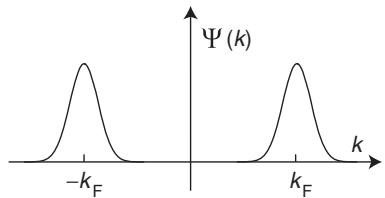
\includegraphics[width=0.5\textwidth]{figs/ch10/fig_10.2.jpg}
\caption*{图 10.2\quad 费米子场的傅里叶分量。在玻色化步骤中，我们只保留费米子场在 $\pm k_{\mathrm{F}}$ 处的动量分量。}\label{fig:auto:10.2}
\end{figure}

然而，负能量态给卢廷格模型引入了一个微妙的复杂性。基态中，右移态的负动量支与左移态的正动量支被占据。这一点画在图 10.1(c) 中，可以看作是负能量狄拉克海的填充。这里的类比是狄拉克理论中的正电子态与卢廷格模型中的负能量单粒子态。然而，哈密顿量式 (10.6) 是用作用在零粒子态空间上的、右移场与左移场的产生算符 $\Psi_{\sigma\pm}^{\dagger}$ 表示的。在这个空间里，电子之间的相互作用项为零。换句话说，我们的哈密顿量缺少基态能量。卢廷格（L1960）通过对左移场与右移场实施如下形式的正则变换
\begin{equation*}
\Psi_{\sigma+}(k)\to
\begin{cases}
b_{k\sigma}, & k\geqslant 0,\\
c_{k\sigma}^{\dagger}, & k<0,
\end{cases}
\tag{10.8}
\end{equation*}
\begin{equation*}
\Psi_{\sigma-}(k)\to
\begin{cases}
b_{k\sigma}, & k<0,\\
c_{k\sigma}^{\dagger}, & k\geqslant 0,
\end{cases}
\tag{10.9}
\end{equation*}
实际填满了负能量狄拉克海。$b_{k\sigma}$ 与 $c_{k\sigma}$ 服从通常的反对易关系。算符 $\Psi_{\sigma+}(k)$（它湮灭一个动量为 $k$ 的右移电子）作用在填满的费米海上，对应于 $k>0$ 时湮灭一个电子，而 $k<0$ 时产生一个空穴。这个变换的一个后果是：动量态 $k$ 中的元激发是由一个粒子与一个空穴组成的对激发。而且，正是这些激发的线性组合，现在描述电子气的集体激发或等离体激发。然而，卢廷格并不知道这个正则变换同时也改变了涉及电子密度的对易子的值。这正是该正则变换给卢廷格模型带来的深刻变化。马蒂斯（Mattis）和利布（Lieb）（ML1965）最先指出这一点，并正确地求解了卢廷格模型。

为了说明这种基底切换所引入的变化，我们用新的粒子–空穴算符改写哈密顿量。变换后的自由哈密顿量
\begin{equation*}
H_{\mathrm{F}}=\hbar v_{\mathrm{F}}\int_{-\infty}^{\infty}|p|\,\mathrm{d}p\left[b_{p}^{\dagger}b_{p}+c_{p}^{\dagger}c_{p}\right]+W,
\tag{10.10}
\end{equation*}
含有常数
\begin{equation*}
W=-\hbar v_{\mathrm{F}}\int_{0}^{\infty}p\,\mathrm{d}p+\hbar v_{\mathrm{F}}\int_{-\infty}^{0}p\,\mathrm{d}p,
\tag{10.11}
\end{equation*}
它代表填满的狄拉克海的无穷大能量。这个结果本来也可以通过把原哈密顿量中的算符正规排序（normal-ordering）得到。考虑一个任意参考态 $|\Omega\rangle$ 和一个可以写成产生与湮灭算符之积的算符 $\hat{A}$。把 $\hat{A}$ 中的产生与湮灭算符正规排序，意思是把所有产生算符移到最左边、把所有湮灭算符移到最右边。这样一来，由对易子产生的无穷大量就被消除了。我们用记号 $:\hat{A}:$ 表示正规排序。于是 $:\hat{A}:|\Omega\rangle=0$，而且 $:\hat{A}:$ 相对于基态 $|\Omega\rangle$ 的任何平均恒为零，即 $\langle\Omega|:\hat{A}:|\Omega\rangle=0$。因此，式 (10.8) 中的变换等价于相对于填满的狄拉克海对左右移场算符作正规排序。这样做，便能把填满的负能量态的无穷大能量提取出来。

我们再来看右移子与左移子密度的动量表象：
\begin{align*}
n_{\sigma\pm}(x)&=\Psi_{\sigma\pm}^{\dagger}(x)\Psi_{\sigma\pm}(x)\\
&=\int_{-\infty}^{\infty}\frac{\mathrm{d}p}{2\pi}\frac{\mathrm{d}q}{2\pi}\Psi_{\sigma\pm}^{\dagger}(p)\Psi_{\sigma\pm}(q)\mathrm{e}^{\mathrm{i}(q-p)x}
\tag{10.12}
\end{align*}
其中
\begin{equation*}
n_{\sigma\pm}(q)=\int_{-\infty}^{\infty}\mathrm{d}x\,\mathrm{e}^{-\mathrm{i}qx}n_{\sigma\pm}(x).
\tag{10.13}
\end{equation*}
把变换后的左移、右移形式代入式 (10.12)，并（按照式 (10.13)）作傅里叶变换，我们发现 $n_{\sigma\pm}(k)$ 的形式
\begin{gather*}
n_{\sigma+}(k>0)=\int_{0}^{\infty}\frac{\mathrm{d}q}{2\pi}\left[b_{q}^{\dagger}b_{k+q}+c_{-k-q}c_{-q}^{\dagger}+c_{-q}b_{k-q}\,\theta(k-q)\right],\\
n_{\sigma+}(k<0)=\int_{0}^{\infty}\frac{\mathrm{d}q}{2\pi}\left[b_{k-q}^{\dagger}b_{q}+c_{-q}c_{k-q}^{\dagger}+b_{q}^{\dagger}c_{k+q}^{\dagger}\,\theta(-k-q)\right],\\
n_{\sigma-}(k>0)=\int_{0}^{\infty}\frac{\mathrm{d}q}{2\pi}\left[b_{-k-q}^{\dagger}b_{-q}+c_{q}c_{k+q}^{\dagger}+b_{-q}^{\dagger}c_{k-q}^{\dagger}\,\theta(k-q)\right],\\
n_{\sigma-}(k<0)=\int_{0}^{\infty}\frac{\mathrm{d}q}{2\pi}\left[b_{-q}^{\dagger}b_{k-q}+c_{q-k}c_{q}^{\dagger}+c_{q}b_{k+q}\,\theta(-k-q)\right],
\end{gather*}
依赖于动量的符号。这里导出的密度动量分量的形式，与马蒂斯和利布（ML1965）给出的形式等价。差别源于式 (10.13) 中密度傅里叶变换的定义。密度对动量符号的依赖，来源于基本激发的成对性质。

也正是在这个复杂性中，在原来的左右移基底与粒子–空穴基底中计算某些对易子时出现了差别。考虑总电子密度的流算符
\begin{equation*}
j_{0}^{\sigma}=\Psi_{\sigma+}^{\dagger}(x)\Psi_{\sigma+}(x)+\Psi_{\sigma-}^{\dagger}(x)\Psi_{\sigma-}(x)
\tag{10.14}
\end{equation*}
以及电子密度之差
\begin{equation*}
j_{1}^{\sigma}=\hbar v_{\mathrm{F}}\left(\Psi_{\sigma+}^{\dagger}(x)\Psi_{\sigma+}(x)-\Psi_{\sigma-}^{\dagger}(x)\Psi_{\sigma-}(x)\right)
\tag{10.15}
\end{equation*}
在原来的左右移基底中，涉及 $j_{0}^{\sigma}$ 与 $j_{1}^{\sigma}$ 的对易子恒为零。然而，如果采用新的粒子–空穴基底（式 (10.8)），我们发现流的各分量之间的等时对易关系
\begin{equation*}
\left[j_{0}^{\sigma}(x),j_{1}^{\sigma}(y)\right]=-\frac{\mathrm{i}\hbar v_{\mathrm{F}}}{\pi}\partial_{x}\delta(x-y),
\tag{10.16}
\end{equation*}
\begin{equation*}
\left[j_{0}^{\sigma}(x),j_{0}^{\sigma}(y)\right]=\left[j_{1}^{\sigma}(x),j_{1}^{\sigma}(y)\right]=0,
\tag{10.17}
\end{equation*}
服从玻色统计。第一个对易子的右端是一个 c 数。这一分歧有点令人惊讶，但如果我们把密度写成一次量子化的形式
\begin{equation*}
n_{\sigma\pm}(k)=\int_{-\frac{L}{2}}^{\frac{L}{2}}\mathrm{d}x\,\mathrm{e}^{-\mathrm{i}kx},
\tag{10.18}
\end{equation*}
它并非完全出乎意料。这些分量平凡地对易。然而，当狄拉克海被填满时，这并不是密度算符在物理上相关的形式。施温格（Schwinger，S1959）早就预见到了这个表观佯谬：基态的存在本身就迫使某些对易子非零，而它们在一次量子化语言中本会平凡地恒为零。对卢廷格模型的全部后果，由马蒂斯和利布（ML1965）给出。

\section{卢廷格模型的玻色化}

在求解完整的卢廷格模型之前，先考虑一个集中体现玻色化步骤若干特征的简单例子是不无益处的。考虑 $H_{\mathrm{F}}$ 的一个无自旋版本，其场为 $\Psi_{n}$。我们同时在每个格点 $n$ 上引入标准的泡利自旋算符 $\sigma_{n}^{x,y,z}$；这些算符在不同格点上相互对易，因而是玻色算符。这些自旋与电子自旋没有物理上的关联；它们只是为玻色算符提供了一个方便的表示。$H_{\mathrm{F}}$ 的玻色化可以通过取
\begin{equation*}
\Psi_{n}=\frac{1}{2}\prod_{m<n}\sigma_{m}^{z}\left(\sigma_{n}^{x}+\mathrm{i}\sigma_{n}^{y}\right).
\tag{10.19}
\end{equation*}
来实现。$\Psi_{n}$ 所服从的反对易关系由这条玻色算符链（所谓的\emph{约当–维格纳弦}（Jordan–Wigner string））来保证。相应的玻色哈密顿量可以由式 (10.19) 与 $H_{\mathrm{F}}$ 得到，为
\begin{equation*}
H_{\mathrm{B}}=\sum_{n}-\frac{t}{2}\left(\sigma_{n}^{x}\sigma_{n+1}^{x}+\sigma_{n}^{y}\sigma_{n+1}^{y}\right)-\frac{\mu}{2}\sigma_{n}^{z}.
\tag{10.20}
\end{equation*}
费米子描述与玻色描述之间的等价性体现在多个方面，并预示了卢廷格模型的若干类似结果。$\Psi_{n}$ 及其玻色对应物所服从的运动方程是等价的。至关重要的是，在两种表示中得到的关联函数相同（参见式 (10.47) 与式 (10.51)、(10.52)）。

现在我们转向构造卢廷格模型自由部分的等价玻色理论。为此，我们关注海森堡运动方程
\begin{equation*}
-\mathrm{i}\partial_{t}j_{0}^{\sigma}(x)=\left[H_{\mathrm{F}},j_{0}^{\sigma}(x)\right].
\tag{10.21}
\end{equation*}
结果表明，式 (10.21) 中对易子的值与狄拉克海的填充无关。也就是说，与那些涉及密度分量的对易子不同，这个对易子在正规排序下不变。左移子与右移子的密度同自由哈密顿量的对易子
\begin{align*}
\left[H_{\mathrm{F}},n_{\sigma+}(\pm k)\right]&=\mp k\,n_{\sigma+}(\pm k),\\
\left[H_{\mathrm{F}},n_{\sigma-}(\pm k)\right]&=\pm k\,n_{\sigma-}(\pm k),
\tag{10.22}
\end{align*}
依赖于动量的符号。注意，相对于马蒂斯和利布的结果，这里有一个符号改变。此处的差别同样源于我们式 (10.13) 中傅里叶变换的定义。于是
\begin{align*}
\biggl[H_{\mathrm{F}},\int_{-\infty}^{\infty}\mathrm{d}q\,\mathrm{e}^{\mathrm{i}qx}j_{0}^{\sigma}(q)\biggr]&=\hbar v_{\mathrm{F}}\int_{0}^{\infty}\mathrm{d}q\,\mathrm{e}^{\mathrm{i}qx}q\left(n_{\sigma-}(q)-n_{\sigma+}(q)\right)\\
&\quad+\hbar v_{\mathrm{F}}\int_{0}^{\infty}\mathrm{d}q\,\mathrm{e}^{-\mathrm{i}qx}q\left(n_{\sigma+}(-q)-n_{\sigma-}(-q)\right)\\
&=\hbar v_{\mathrm{F}}\int_{-\infty}^{\infty}\mathrm{d}q\,\mathrm{e}^{\mathrm{i}qx}q\left(n_{\sigma-}(q)-n_{\sigma+}(q)\right)\\
&=\mathrm{i}\partial_{x}j_{1}^{\sigma}
\tag{10.23}
\end{align*}
或者等价地
\begin{equation*}
\partial_{t}j_{0}^{\sigma}=-\partial_{x}j_{1}^{\sigma}.
\tag{10.24}
\end{equation*}

如果引入记号 $t\to x_{0}$ 与 $x\to x_{1}$，并记 $x\equiv(x_{0},x_{1})$，就可以把海森堡运动方程改写成一个守恒方程：
\begin{equation*}
\partial_{\mu}j_{\mu}^{\sigma}=0.
\tag{10.25}
\end{equation*}
于是，相对于整个狄拉克海正规排序的总费米流是守恒的。

费米流的守恒提示我们：如果定义一个玻色场 $\Phi_{\sigma}(x)$ 及其共轭动量 $\Pi_{\sigma}(x)$，使得
\begin{equation*}
j_{0}^{\sigma}(x)=\frac{1}{\sqrt{\pi}}\partial_{x}\Phi_{\sigma}(x)
\tag{10.26}
\end{equation*}
以及
\begin{equation*}
j_{1}^{\sigma}(x)=-\frac{1}{\sqrt{\pi}}\partial_{t}\Phi_{\sigma}(x)=-\frac{1}{\sqrt{\pi}}\Pi_{\sigma}(x),
\tag{10.27}
\end{equation*}
则海森堡运动方程
\begin{equation*}
\partial_{t}\left[\partial_{x}\Phi_{\sigma}(x)\right]=\partial_{x}\Pi_{\sigma}(x),
\tag{10.28}
\end{equation*}
将类似于两个共轭场的运动方程。为满足流的玻色统计，要求
\begin{equation*}
\left[\Phi_{\sigma}(x),\Pi_{\sigma'}(y)\right]=\mathrm{i}\delta_{\sigma\sigma'}\delta(x-y).
\tag{10.29}
\end{equation*}
在玻色基底中，自由哈密顿量密度
\begin{equation*}
H_{\mathrm{F}}=\frac{\hbar v_{\mathrm{F}}}{2}\sum_{\sigma}\int\mathrm{d}x\left[\Pi_{\sigma}^{2}(x)+\left(\partial_{x}\Phi_{\sigma}(x)\right)^{2}\right],
\tag{10.30}
\end{equation*}
给出的运动方程，与费米基底中密度的海森堡演化方程等价。这样，我们就把费米子理论重新表述成了一个等价的玻色理论。我们强调，这个玻色理论是通过基于运动方程的类比构造出来的。因此，式 (10.30) 并不是等价玻色哈密顿量密度的唯一选择。所谓构造一个等价的玻色理论，我们指的仅仅是两种表述中运动方程之间的等价。

我们还可以把玻色化步骤再向前推进一步，显式地构造费米场 $\Psi_{\sigma\pm}(x)$ 与新玻色场 $\Phi_{\sigma}(x)$ 之间的映射。这样的映射存在麻烦，因为玻色场描述的是涉及两个费米算符的粒子–空穴激发。于是，改变电子数的过程被禁止。眼下我们把这个难题搁置一旁，先来发展一个涉及玻色场、并保持费米场反对易关系的映射。玻色化的关键想法是：把左移与右移费米场同如下形式的玻色场\emph{相联系}（而非\emph{相等}）：
\begin{align*}
\Psi_{\sigma\pm}(x)&=\frac{1}{\sqrt{2\pi a}}\mathrm{e}^{-\mathrm{i}\sqrt{\pi}\left[\int_{-\infty}^{x}\Pi_{\sigma}(x')\,\mathrm{d}x'\mp\Phi_{\sigma}(x)\right]}\\
&=\frac{1}{\sqrt{2\pi a}}\mathrm{e}^{\pm\mathrm{i}\sqrt{\pi}\Phi_{\sigma\pm}(x)},
\tag{10.31}
\end{align*}
其中
\begin{equation*}
\Phi_{\sigma\pm}(x)=\Phi_{\sigma}(x)\mp\int_{-\infty}^{x}\Pi_{\sigma}(x')\,\mathrm{d}x'.
\tag{10.32}
\end{equation*}
至关重要的是，算符等价关系式 (10.31) 必须严格在正规排序的意义上理解。例如，如果把式 (10.31) 朴素地代入哈密顿量的连续版本（式 (10.6)），得到的玻色哈密顿量将对应于式 (10.30) 的两倍。这样的方程会给出错误的运动方程。这更凸显了我们的声明：费米场应当与玻色场（式 (10.31)）相联系，而非相等。只有当计算物理可观察量的平均值时，两种理论之间才出现真正的等式。式 (10.31) 的物理动机如下。粒子位于 $x$ 处的振幅是 $\Psi_{\sigma\pm}(x)$。经典上，把粒子从 $x$ 平移到 $x+a$ 由位移算符 $\mathrm{e}^{a\partial_{x}}$ 实现；量子力学上，这个量变成动量算符的指数。因此，$\Psi_{\sigma\pm}(x)$ 必须正比于动量算符的指数，我们把这个量记为 $\Pi_{\sigma}(x)$。然而，如果只有这一层依赖关系，$\Psi_{\sigma\pm}(x)$ 将与自身对易。指数形式是能保证费米子反对易关系（式 (10.31)）的最简单形式。

为了解决玻色化形式的费米场（就其现有形式而言）无法连接粒子数不同的电子态这一问题，我们引入按整数改变粒子数的阶梯算符（KS1996；H1981）。这样的阶梯算符（传统上称为“克莱因因子”（Klein factors））必须位于玻色算符的空间之外，因为玻色子必然是偶数个费米子的复合体。玻色算符的任何组合都绝不可能产生单个电子。令 $N_{\sigma}$ 表示电子占据数相对其基态值的偏离。按照科特利亚尔（Kotliar）和 Si（KS1996）的记号，我们引入算符 $F_{\sigma}$（$F_{\sigma}^{\dagger}$），它使 $N_{\sigma}$ 减少（增加）1。对 $q\neq 0$，$F_{\sigma}$ 与 $\Psi_{\sigma\pm}$ 中的所有玻色场对易。因此，$F_{\sigma}$ 与 $N_{\sigma}$ 代表电子气的零动量模式；$q\neq 0$ 的模式是粒子–空穴激发。$F_{\sigma}$ 的附加对易关系为
\begin{align*}
&F_{\sigma}^{\dagger}F_{\sigma}=F_{\sigma}F_{\sigma}^{\dagger}=1,\\
&F_{\sigma}^{\dagger}F_{\sigma'}=-F_{\sigma'}F_{\sigma}^{\dagger},\\
&F_{\sigma}F_{\sigma'}=-F_{\sigma'}F_{\sigma}.
\tag{10.33}
\end{align*}
电子的物理态现在由
\begin{equation*}
\tilde{\Psi}_{\sigma\pm}^{\dagger}(x)=F_{\sigma}^{\dagger}\mathrm{e}^{\frac{2\pi\mathrm{i}xN_{\sigma}}{L}}\Psi_{\sigma\pm}^{\dagger}.
\tag{10.34}
\end{equation*}
捕捉。对于不守恒粒子数的过程，必须把“克莱因因子”包括进来（KS1996；H1981；VDS1998）。然而，由于我们关注的问题都守恒粒子数，我们将略去“克莱因因子”，因为它们不能改变物理。尽管如此，它们是玻色化完整故事的一部分。

现在我们转向相互作用项的玻色化。在连续极限下，哈伯德相互作用可以写成
\begin{equation*}
H_{U}=aU\int_{-L/2}^{L/2}\mathrm{d}x\left(R_{\uparrow}^{\dagger}(x)+L_{\uparrow}^{\dagger}(x)\right)\left(R_{\uparrow}(x)+L_{\uparrow}(x)\right)\left(R_{\downarrow}^{\dagger}(x)+L_{\downarrow}^{\dagger}(x)\right)\left(R_{\downarrow}(x)+L_{\downarrow}(x)\right),
\tag{10.35}
\end{equation*}
其中 $R_{\sigma}(x)(L_{\sigma}(x))=\Psi_{n\sigma\pm}\mathrm{e}^{\pm\mathrm{i}k_{\mathrm{F}}x}/\sqrt{a}$。为了实施玻色化方案，必须对哈伯德相互作用中的算符作正规排序。与自由系统一样，对哈伯德相互作用中的算符作正规排序，
\begin{equation*}
H_{U}=:H_{U}:+Q,
\tag{10.36}
\end{equation*}
会生成一个常数项（$Q$），它又是无穷大。此时，无穷大项与负能量态中的无穷大电荷相联系。这里的关键在于，无穷大项是常数，因此可以忽略。

现在把式 (10.35) 展开，只保留非振荡项，就会发现哈伯德相互作用约化为
\begin{align*}
H_{U}\to H_{\mathrm{int}}=aU\int_{-L/2}^{L/2}\mathrm{d}x\Big[&\left(:\Psi_{\uparrow+}^{\dagger}\Psi_{\uparrow+}:+:\Psi_{\uparrow-}^{\dagger}\Psi_{\uparrow-}:\right)\left(:\Psi_{\downarrow+}^{\dagger}\Psi_{\downarrow+}:+:\Psi_{\downarrow-}^{\dagger}\Psi_{\downarrow-}:\right)\\
&+\left[:\Psi_{\uparrow+}^{\dagger}\Psi_{\uparrow-}::\Psi_{\downarrow-}^{\dagger}\Psi_{\downarrow+}:+\mathrm{h.c.}\right]\Big].
\tag{10.37}
\end{align*}
图 10.3 画出了 $H_{\mathrm{int}}$ 中保留的两类散射过程。在图 10.3(a) 中，每个顶点上净的动量转移为零。因此，式 (10.37) 的第一项对应电子的前向散射（forward scattering）。在第二项中（见图 10.3(b)），粒子从左（右）移子被转化为右（左）移子。因此，这一项对应一个背散射（backscattering）过程。我们丢掉了带 $\mathrm{e}^{\pm\mathrm{i}4k_{\mathrm{F}}}$ 前因子的项。半填充时 $k_{\mathrm{F}}=\pi/2$，指数前因子化为 1。$4k_{\mathrm{F}}$ 项被称为 Umklapp 过程（倒逆过程），在其中两个右（左）移子被湮灭，同时产生两个左（右）移子。稍后我们会回到这些项。

为了完成玻色化方案，我们需要一条规则，把式 (10.37) 中费米算符的乘积用玻色场写出来。为此，我们使用贝克–豪斯多夫（Baker–Hausdorff）恒等式
\begin{equation*}
\mathrm{e}^{A}\mathrm{e}^{B}=\mathrm{e}^{A+B}\mathrm{e}^{\frac{1}{2}[A,B]}.
\tag{10.38}
\end{equation*}

\begin{figure}[H]\centering
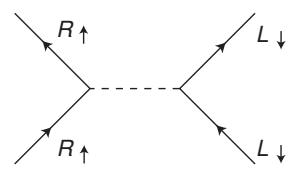
\includegraphics[width=0.32\textwidth]{figs/ch10/fig_10.3_a.jpg}\hfill
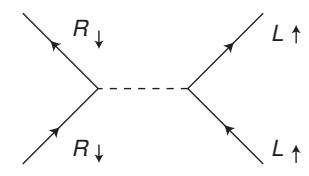
\includegraphics[width=0.32\textwidth]{figs/ch10/fig_10.3_b.jpg}\\[2pt]
{\small (a)}\\[12pt]
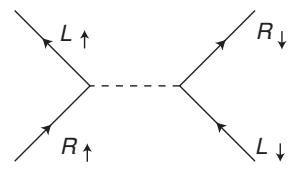
\includegraphics[width=0.32\textwidth]{figs/ch10/fig_10.3_c.jpg}\hfill
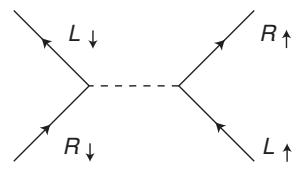
\includegraphics[width=0.32\textwidth]{figs/ch10/fig_10.3_d.jpg}\\[2pt]
{\small (b)}
\caption*{图 10.3\quad (a) 对应式 (10.37) 第一项的前向散射过程。R(L) 代表右移场与左移场。在前向散射项的每个顶点处，动量改变为零。虚线表示库仑相互作用 $aU$。(b) 背散射对应式 (10.37) 的第二项。每个顶点处动量改变的大小为 $|2k_{\mathrm{F}}|$。}\label{fig:auto:10.3}
\end{figure}

利用对易关系式 (10.29)，我们把背散射项中的算符乘积
\begin{equation*}
\Psi_{\sigma+}^{\dagger}\Psi_{\sigma-}=\frac{1}{2\pi a}\mathrm{e}^{-\mathrm{i}\sqrt{4\pi}\Phi_{\sigma}(x)}\mathrm{e}^{-\pi\mathrm{i}/2}=-\mathrm{i}\frac{1}{2\pi a}\mathrm{e}^{-\mathrm{i}\sqrt{4\pi}\Phi_{\sigma}(x)}
\tag{10.39}
\end{equation*}
约化为玻色场的简单指数。$-\mathrm{i}$ 这个因子来自对易子
\begin{align*}
\left[\Phi_{\sigma+}(x),\Phi_{\sigma-}(y)\right]&=\left[\Phi_{\sigma}(x),\int_{-\infty}^{y}\Pi(x')\,\mathrm{d}x'\right]+\left[\Phi_{\sigma}(y),\int_{-\infty}^{x}\Pi_{\sigma}(x')\,\mathrm{d}x'\right]\\
&=\mathrm{i}\int_{-\infty}^{y}\mathrm{d}x'\,\delta(x-x')+\mathrm{i}\int_{-\infty}^{x}\mathrm{d}x'\,\delta(y-x')\\
&=\mathrm{i}.
\tag{10.40}
\end{align*}
进一步的化简需要一些附加的恒等式。费米场 $\Psi_{\sigma\pm}$ 是两个服从玻色统计的场的指数。仿照谐振子，我们把指数拆分成产生算符部分与湮灭算符部分之和。于是，$\Psi_{\sigma\pm}$ 场具有如下形式
\begin{equation*}
\Psi_{\sigma\pm}=\mathrm{e}^{A}=\mathrm{e}^{A^{+}+A^{-}},
\tag{10.41}
\end{equation*}
其中 $A^{+}$（$A^{-}$）代表 $A$ 的产生（湮灭）算符部分。利用贝克–豪斯多夫算符恒等式（式 (10.38)），我们发现
\begin{equation*}
\mathrm{e}^{A}=\mathrm{e}^{A^{+}}\mathrm{e}^{A^{-}}\mathrm{e}^{-\frac{1}{2}[A^{+},A^{-}]}.
\tag{10.42}
\end{equation*}
由于正规排序把所有产生算符置于左边、湮灭算符置于右边，
\begin{equation*}
:\mathrm{e}^{A}:\ \equiv\ \mathrm{e}^{A^{+}}\mathrm{e}^{A^{-}}=\mathrm{e}^{A}\mathrm{e}^{\frac{1}{2}[A^{+},A^{-}]}
\tag{10.43}
\end{equation*}
就是 $\Psi_{\sigma\pm}$ 场相应的正规排序形式。这个表达式在玻色化步骤中极为有用。例如，文献中（M1975）常把左移与右移费米场写成正规排序的形式。正规排序形式与式 (10.31) 相差式 (10.43) 中的相位因子。就背散射项而言，我们可以用式 (10.43) 计算两个正规排序算符的乘积。把式 (10.43) 连用两次，我们发现
\begin{equation*}
:\mathrm{e}^{A}::\mathrm{e}^{B}:=\mathrm{e}^{[A^{-},B^{+}]}:\mathrm{e}^{A+B}:,
\tag{10.44}
\end{equation*}
其中 $[A^{\pm},B^{\pm}]=0$。一般地，$[A^{\pm},B^{\mp}]$ 是一个 c 数。对 $\Phi_{\sigma+}=A$、$\Phi_{\sigma-}=B$ 的情形，式 (10.44) 指数因子中的对易子已由马蒂斯（M1974）和曼德尔斯坦（Mandelstam，M1975）算出，其值为 1。于是
\begin{equation*}
:\Psi_{\uparrow+}^{\dagger}\Psi_{\uparrow-}::\Psi_{\downarrow-}^{\dagger}\Psi_{\downarrow+}:+\mathrm{h.c.}=\frac{1}{2\pi^{2}a^{2}}:\cos\left(\sqrt{4\pi}\left(\Phi_{\uparrow}(x)-\Phi_{\downarrow}(x)\right)\right):.
\tag{10.45}
\end{equation*}

前向散射项要稍难一些，因为 $\Psi_{\uparrow+}^{\dagger}(x+\epsilon)\Psi_{\uparrow+}(x-\epsilon)$ 这种形式的算符乘积在 $\epsilon\to 0$ 的极限下没有良好的定义。天真地想，人们或许预期这个量等于 1，实则不然。我们可以通过考察费米子关联函数
\begin{align*}
\left\langle\Psi_{\sigma+}^{\dagger}(x)\Psi_{\sigma+}(0)\right\rangle&=\int_{-\infty}^{\infty}\frac{\mathrm{d}k}{2\pi}\int_{-\infty}^{\infty}\frac{\mathrm{d}q}{2\pi}\mathrm{e}^{-\mathrm{i}qx}\left\langle\Psi_{\sigma+}^{\dagger}(q)\Psi_{\sigma+}(k)\right\rangle\\
&=\int_{0}^{\infty}\frac{\mathrm{d}k}{2\pi}\mathrm{e}^{\mathrm{i}kx}.
\tag{10.46}
\end{align*}
来计算这个乘积。也就是说，双重积分收缩为 $2\pi\delta(k-q)$，且 $k<0$。后一约束来源于右移子在基态中只存在于负动量态。式 (10.46) 在大动量处行为不佳，但可以通过引入指数因子 $\mathrm{e}^{-ak}$ 使之正规化，其中晶格常数充当短距离截断。于是我们得到
\begin{equation*}
\left\langle\Psi_{\sigma+}^{\dagger}(x)\Psi_{\sigma+}(0)\right\rangle=\frac{1}{2\pi}\frac{1}{a-\mathrm{i}x}.
\tag{10.47}
\end{equation*}
对于左移子，相应的关联函数是式 (10.47) 的复共轭。

如果我们用这些场算符的玻色化形式去计算密度关联函数，就必须得到相同的结果。为此，我们利用式 (10.38) 与 (10.44) 化简形如 $\mathrm{e}^{A}\mathrm{e}^{B}$ 的乘积：
\begin{equation*}
\mathrm{e}^{A}\mathrm{e}^{B}=:\mathrm{e}^{A+B}:\,\mathrm{e}^{[A^{-},B^{+}]+\frac{[A^{-},A^{+}]+[B^{-},B^{+}]}{2}}.
\tag{10.48}
\end{equation*}
一般地，式 (10.48) 中出现的对易子都是 c 数。此外，由于 $\langle(A^{\pm})^{2}\rangle=\langle A^{+}A^{-}\rangle=0$，立即有 $\langle[A^{-},A^{+}]\rangle=\langle A^{2}\rangle$。于是
\begin{equation*}
\langle\mathrm{e}^{A}\mathrm{e}^{B}\rangle=\langle:\mathrm{e}^{A+B}:\rangle\,\mathrm{e}^{\langle AB+\frac{A^{2}+B^{2}}{2}\rangle}.
\tag{10.49}
\end{equation*}
任何正规排序算符之指数的平均值都是 1，即 $\langle:\mathrm{e}^{A}:\rangle=1$。这样，我们就得到了计算关联函数的至关重要的规则
\begin{equation*}
\langle\mathrm{e}^{A}\mathrm{e}^{B}\rangle=\mathrm{e}^{\langle AB+\frac{A^{2}+B^{2}}{2}\rangle},
\tag{10.50}
\end{equation*}
由此可得
\begin{equation*}
\left\langle\Psi_{\sigma+}^{\dagger}(x)\Psi_{\sigma+}(0)\right\rangle=\frac{1}{2\pi a}\mathrm{e}^{\pi\left\langle\Phi_{\sigma+}(x)\Phi_{\sigma+}(0)-\Phi_{\sigma+}^{2}(0)\right\rangle}.
\tag{10.51}
\end{equation*}
通过与式 (10.47) 类比，我们求得
\begin{align*}
\left\langle\Psi_{\sigma+}^{\dagger}(x)\Psi_{\sigma+}(0)\right\rangle&=\frac{1}{2\pi a}\mathrm{e}^{\pi G_{+}(x)}\\
&=\frac{1}{2\pi a}\frac{a}{a-\mathrm{i}x}
\tag{10.52}
\end{align*}
或者等价地
\begin{equation*}
\langle\mathrm{e}^{-\mathrm{i}\eta\Phi_{\sigma\pm}}\mathrm{e}^{\mathrm{i}\eta\Phi_{\sigma\pm}}\rangle=\left(\frac{a}{a\mp\mathrm{i}x}\right)^{\eta^{2}/\pi}\equiv\mathrm{e}^{\eta^{2}G_{\pm}}.
\tag{10.53}
\end{equation*}

现在我们拥有了计算最初那个费米子乘积的工具：
\begin{align*}
:\Psi_{\sigma\pm}^{\dagger}(x)\Psi_{\sigma\pm}(x):&=\lim_{\epsilon\to 0}\frac{1}{2\pi a}:\mathrm{e}^{\mp\mathrm{i}\sqrt{\pi}\left(\Phi_{\sigma\pm}(x+\epsilon)\pm\Phi_{\sigma\pm}(x-\epsilon)\right)}:\ \mathrm{e}^{\pi G_{\pm}}\\
&=\lim_{\epsilon\to 0}\frac{1}{2\pi a}:1\mp 2\mathrm{i}\sqrt{\pi}\,\partial_{x}\Phi_{\sigma\pm}\,\epsilon+\cdots:\left(\pm\frac{\mathrm{i}a}{2\epsilon\pm\mathrm{i}a}\right)\\
&=\lim_{\epsilon\to 0}\frac{\pm\mathrm{i}}{2\pi(2\epsilon\pm\mathrm{i}a)}+:\frac{1}{2\sqrt{\pi}}\partial_{x}\Phi_{\sigma\pm}+O(\epsilon):.
\tag{10.54}
\end{align*}
对任意小的 $a$，此表达式中的第一项是无穷大，这反映出负能量态中右移子与左移子的数目无穷多。把电荷密度中的算符正规排序，会消除基态中发散的电荷密度。因此，正规排序后的电荷密度
\begin{equation*}
:\Psi_{\sigma\pm}^{\dagger}(x)\Psi_{\sigma\pm}(x):=\frac{1}{2\sqrt{\pi}}\partial_{x}\Phi_{\sigma\pm}(x)
\tag{10.55}
\end{equation*}
在玻色基底中具有良好的定义。注意到
\begin{equation*}
:\Psi_{\sigma+}^{\dagger}(x)\Psi_{\sigma+}(x):+:\Psi_{\sigma-}^{\dagger}(x)\Psi_{\sigma-}(x):=\frac{1}{\sqrt{\pi}}:\partial_{x}\Phi_{\sigma}(x):
\tag{10.56}
\end{equation*}
并利用式 (10.45)，我们把相互作用项化简为
\begin{equation*}
H_{\mathrm{int}}=aU\int\mathrm{d}x\sum_{\sigma}\left[\frac{:\partial_{x}\Phi_{\uparrow}\partial_{x}\Phi_{\downarrow}:}{\pi}+\frac{1}{2\pi^{2}a^{2}}:\cos\left(\sqrt{4\pi}\left(\Phi_{\uparrow}(x)-\Phi_{\downarrow}(x)\right)\right):\right].
\tag{10.57}
\end{equation*}

通过引入电荷玻色场 $\Phi_{\mathrm{c}}$ 与自旋玻色场 $\Phi_{\mathrm{s}}$，
\begin{equation*}
\Phi_{\mathrm{c}}=\frac{\Phi_{\uparrow}+\Phi_{\downarrow}}{\sqrt{2}},\qquad\Phi_{\mathrm{s}}=\frac{\Phi_{\uparrow}-\Phi_{\downarrow}}{\sqrt{2}},
\tag{10.58}
\end{equation*}
这个表达式以及玻色化步骤的效用便清晰起来。新的电荷场与自旋场服从通常的玻色对易关系，因为它们不过是玻色场的和与差。把这些表达式代入哈密顿量的玻色化部分，我们得到一个哈密顿量 $H_{\mathrm{B}}=H_{\mathrm{c}}+H_{\mathrm{s}}$，其中电荷自由度
\begin{equation*}
H_{\mathrm{c}}=\frac{\hbar v_{\mathrm{F}}}{2}\int\mathrm{d}x\left[\Pi_{\mathrm{c}}^{2}+g_{\mathrm{c}}^{2}(\partial_{x}\Phi_{\mathrm{c}})^{2}\right],
\tag{10.59}
\end{equation*}
与自旋自由度
\begin{equation*}
H_{\mathrm{s}}=\frac{\hbar v_{\mathrm{F}}}{2}\int\mathrm{d}x\left[\Pi_{\mathrm{s}}^{2}+g_{\mathrm{s}}^{2}(\partial_{x}\Phi_{\mathrm{s}})^{2}\right]+\frac{U}{2\pi^{2}a}\int\mathrm{d}x:\cos\sqrt{8\pi}\,\Phi_{\mathrm{s}}:,
\tag{10.60}
\end{equation*}
完全解耦。耦合常数
\begin{equation*}
g_{\mathrm{c}}^{2}=1+\frac{aU}{2\pi\hbar v_{\mathrm{F}}}
\tag{10.61}
\end{equation*}
与
\begin{equation*}
g_{\mathrm{s}}^{2}=1-\frac{aU}{2\pi\hbar v_{\mathrm{F}}},
\tag{10.62}
\end{equation*}
现在是相互作用的函数，可以用它们为自旋与电荷自由度定义新的速度。令 $v_{\mathrm{F}}^{\mathrm{c}}=v_{\mathrm{F}}g_{\mathrm{c}}$ 与 $v_{\mathrm{F}}^{\mathrm{s}}=v_{\mathrm{F}}g_{\mathrm{s}}$。为了看出自旋部分与电荷部分现在以不同的速度运动，我们考虑变换 $\Phi_{\nu}\sqrt{g_{\nu}}\to\tilde{\Phi}_{\nu}$ 与 $\Pi_{\nu}1/\sqrt{g_{\nu}}\to\tilde{\Pi}_{\nu}$，其中 $\nu=\mathrm{c},\mathrm{s}$。这个变换使玻色对易关系（式 (10.40)）保持不变。用重标度后的场来表示，电荷自由度
\begin{equation*}
H_{\mathrm{c}}=\frac{\hbar v_{\mathrm{F}}^{\mathrm{c}}}{2}\int\mathrm{d}x\left[\tilde{\Pi}_{\mathrm{c}}^{2}+(\partial_{x}\tilde{\Phi}_{\mathrm{c}})^{2}\right]
\tag{10.63}
\end{equation*}
看起来像一群无相互作用的费米子，但带有一个新的费米速度 $v_{\mathrm{F}}^{\mathrm{c}}$，它随在位排斥的增强而增大。在自旋部分，
\begin{equation*}
H_{\mathrm{s}}=\frac{\hbar v_{\mathrm{F}}^{\mathrm{s}}}{2}\int\mathrm{d}x\left[\tilde{\Pi}_{\mathrm{s}}^{2}+(\partial_{x}\tilde{\Phi}_{\mathrm{s}})^{2}\right]+\frac{U}{2\pi^{2}a}\int\mathrm{d}x:\cos\sqrt{8\pi/g_{\mathrm{s}}}\,\tilde{\Phi}_{\mathrm{s}}:,
\tag{10.64}
\end{equation*}
当电子之间是排斥相互作用时，自旋的新速度 $v_{\mathrm{F}}^{\mathrm{s}}$ 落后于电荷自由度的速度。于是，自旋与电荷自由度以完全不同的速度运动。自旋部分与电荷部分的另一个差别是 $:\cos\tilde{\Phi}_{\mathrm{s}}:$ 项。在玻色化语言中，这个因子等价于原费米子哈密顿量中的一个质量项。物理上，质量项代表一个能隙。然而，只有在库仑相互作用为吸引（S1990）、电子形成束缚的反铁磁对的情形下，自旋能隙才会出现，这进一步加大了一维中自旋部分与电荷部分之间的差别。其结果是，对于一维相互作用电子液体，电子分裂成截然不同的自旋与电荷准粒子（实验观察的报道见 (Y2005)）。这样，我们可以把电子看作由两种不同实体组成的复合粒子。我们把携带电荷的那个实体称为空穴子（holon，或称 eon），把自旋部分称为自旋子（spinon）。空穴子（或 eon）与自旋子服从玻色统计。一维中空穴子与自旋子激发的出现，代表着对费米液体行为的显著偏离。在费米液体理论中，相互作用体系与非相互作用体系的激发态之间存在一一对应。一维中的自旋–电荷分离从根本上破坏了这种对应，因为现在电子给出的是两个激发，而不是标志着费米液体理论的那一个激发。

\section{配对束缚：电子单独能做到吗？}

\begin{figure}[H]\centering
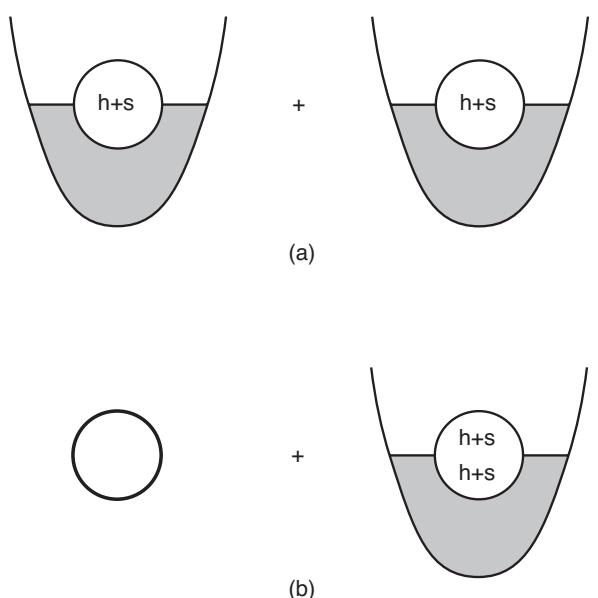
\includegraphics[width=0.5\textwidth]{figs/ch10/fig_10.4.jpg}
\caption*{图 10.4\quad 用于计算 $n=1$ 时配对束缚能的两个电子体系。若 (b) 的能量低于 (a) 的能量，则发生配对束缚。这种局面能否纯粹因电子学的原因而实现，取决于空穴子–空穴子、自旋子–自旋子以及空穴子–自旋子相互作用强度的相对大小。}\label{fig:auto:10.4}
\end{figure}

由科恩（Kohn）与卢廷格的早期论证（见第 9 章）众所周知：当把电子的顶点修正考虑进来时，任何费米体系都具有超导不稳定性（尽管出现在 $10^{-5}$ K 量级的极低温度）。自他们的工作以来，关于超导电性的纯电子机制已有大量论证。我们在这里不提出某个具体的机制，而是借助空穴子–自旋子图像，专注于从纯电子学的角度理解配对束缚（pair binding）的一般思路。令 $\Phi_{n}$ 为含 $n$ 个额外电子的电子体系的能量。配对束缚问题如下：两个各自含 $n+1$ 与 $n-1$ 个额外电子的孤立体系，其总能量是否低于两个各含 $n$ 个额外电子的独立体系？能量差
\begin{equation*}
E_{\mathrm{pair}}^{(n)}=2\Phi_{n}-\Phi_{n+1}-\Phi_{n-1}
\tag{10.65}
\end{equation*}
就是配对束缚能。若 $E_{\mathrm{pair}}^{(n)}>0$，则预期发生配对，因为净吸引有利于歧化（disproportionation）为 $n+1$ 与 $n-1$ 的态。为了说明配对束缚可以仅由排斥相互作用产生，我们采用卢廷格液体的自旋–电荷二分性。为简单起见，考虑 $n=1$ 的情形，如图 10.4 所示。为计算配对束缚能，必须计算 $2\Phi_{1}-\Phi_{2}-\Phi_{0}$。我们取 $\Phi_{0}=0$，并令 $E_{\mathrm{h}}$ 与 $E_{\mathrm{s}}$ 分别为空穴子与自旋子的能量。再定义 $V_{\mathrm{hh}}$ 与 $V_{\mathrm{hs}}$ 为空穴子–空穴子相互作用与空穴子–自旋子相互作用。相关的物理体系画在图 10.4 中。在一个可加常数之内，$2\Phi_{1}$ 的能量
\begin{equation*}
2\Phi_{1}=2\left(E_{\mathrm{h}}+E_{\mathrm{s}}+V_{\mathrm{hs}}\right),
\tag{10.66}
\end{equation*}
就是两个各自添加了一个额外电子的独立电子体系的能量之和，而双重占据态的能量为
\begin{equation*}
\Phi_{2}=2E_{\mathrm{h}}+V_{\mathrm{hh}}+4V_{\mathrm{hs}}+V_{\mathrm{ss}}+2E_{\mathrm{s}}.
\tag{10.67}
\end{equation*}
因子 4 来源于每个电子的两项空穴子–自旋子（holon–spinon）相互作用，再加上两个电子之间的交叉相互作用。我们已假定单态中自旋子的能量为零。这两个态的能量差为
\begin{equation*}
E_{\mathrm{pair}}^{(1)}=-\left(2V_{\mathrm{hs}}+V_{\mathrm{hh}}+V_{\mathrm{ss}}\right),
\tag{10.68}
\end{equation*}
要使单个电子稳定，须有 $V_{\mathrm{hs}}<0$；而库仑定律规定 $V_{\mathrm{hh}}>0$。于是，自旋子–自旋子相互作用能便是决定 $E_{\mathrm{pair}}^{(1)}\lessgtr 0$ 的关键量。在某些情形下，$V_{\mathrm{ss}}$ 恰好具有合适的量值，使得 $E_{\mathrm{pair}}^{(1)}>0$。此时，纯粹排斥性的电子相互作用也能导致配对束缚。

\section{激发谱}

如果将式 (10.63) 与谐振子的标准哈密顿量 $H=P^{2}+Q^{2}$（其中 $P$ 与 $Q$ 为正则动量与坐标）相比较，就会发现玻色化后的电荷部分与一群谐振子等价。正如前文所指出的，卢廷格模型中的电荷激发就是通常的玻色模式，更为人熟知的名称是等离激元激发。这些激发相应的态密度应当是什么？人们或许猜想它们服从标准的玻色–爱因斯坦分布，然而事实并非如此。卢廷格液体（L1960）中的电荷激发，其态密度在费米能级处按 $|k-k_{\mathrm{F}}|^{\alpha}$ 的形式消失，这完全来源于电子之间的关联。该幂律由 $\alpha=(g_{\mathrm{c}}+g_{\mathrm{c}}^{-1})/2-1$ 给出。因此，卢廷格液体并不具有标志费米液体特征的光滑态密度，而是对任何 $U\neq0$ 都会在费米能级处发展出一个软能隙（soft gap）。这一效应的根源可以追溯到电子气的玻色化形式中 $v_{\mathrm{F}}^{\mathrm{c}}$ 被 $g_{\mathrm{c}}$ 重正化。

我们通过计算总电荷关联函数来确立这一结果：
\begin{equation*}
G(x)=\left\langle\sum_{\sigma}\left(\Psi_{\sigma+}(x)\Psi_{\sigma+}^{\dagger}(0)+\Psi_{\sigma-}(x)\Psi_{\sigma-}^{\dagger}(0)\right)\right\rangle.
\tag{10.69}
\end{equation*}
为使记号紧凑，我们定义
\begin{equation*}
\Theta_{\sigma}(x)=\int_{-\infty}^{x}\Pi_{\sigma}(x')\,\mathrm{d}x'.
\tag{10.70}
\end{equation*}

对每个自旋分量，我们作代换 $\Phi_{\uparrow(\downarrow)}=(\Phi_{\mathrm{c}}\pm\Phi_{\mathrm{s}})/\sqrt{2}$ 与 $\Theta_{\uparrow(\downarrow)}=(\Theta_{\mathrm{c}}\pm\Theta_{\mathrm{s}})/\sqrt{2}$，其中上面的符号对应自旋向上，下面的符号对应自旋向下。在没有磁场时，$n_{\uparrow}(x)=n_{\downarrow}(x)$，因而所有对 $\Phi_{\mathrm{s}}$ 或 $\Pi_{\mathrm{s}}$ 线性的平均恒等于零。利用变换后的场 $\tilde{\Phi}_{\nu}(x)$ 与 $\tilde{\Pi}_{\nu}(x)$，我们可以把式 (10.69) 中的平均进一步化简。此时，式 (10.69) 中的平均是对以重正化费米速度 $v_{\mathrm{F}}^{\mathrm{c}}$ 与 $v_{\mathrm{F}}^{\mathrm{s}}$ 为特征的非相互作用玻色化系统的基态取的。于是可以使用化简玻色算符指数函数乘积平均的标准规则。利用 Baker–Hausdorff 恒等式的第三种形式（式 (10.48)），我们发现总电子密度的关联函数化简为
\begin{equation*}
G(x)=\frac{1}{\pi a}\,\mathrm{e}^{\mathrm{i}\,\text{相位}}\,\mathrm{e}^{\frac{\pi}{2}\sum_{\nu=\mathrm{c},\mathrm{s}}\left(g_{\nu}^{-1}a_{\nu}+g_{\nu}b_{\nu}\right)},
\tag{10.71}
\end{equation*}
其中
\begin{equation*}
a_{\nu}=\langle\tilde{\Phi}_{\nu}(x)\tilde{\Phi}_{\nu}(0)-\tilde{\Phi}_{\nu}^{2}(0)\rangle
\tag{10.72}
\end{equation*}
且
\begin{equation*}
b_{\nu}=\langle\tilde{\Theta}_{\nu}(x)\tilde{\Theta}_{\nu}(0)-\tilde{\Theta}_{\nu}^{2}(0)\rangle.
\tag{10.73}
\end{equation*}
相位由交叉项决定。对电荷场与自旋场，交叉项都具有 $\langle\tilde{\Phi}_{\nu}(0)\tilde{\Theta}_{\nu}(0)+\tilde{\Theta}_{\nu}(0)\tilde{\Phi}_{\nu}(0)\rangle-\langle\tilde{\Phi}_{\nu}(x)\tilde{\Theta}_{\nu}(0)+\tilde{\Theta}_{\nu}(x)\tilde{\Phi}_{\nu}(0)\rangle$ 的形式。这一项恒为零（见习题 10.4）。

计算 $G(x)$ 中各平均的最简单办法是引入自由玻色场的傅里叶展开\footnote{译注：原书式 (10.74) 中两处算符的宗量印作 $\phi_{\nu}(x)$，按式 (10.75) 的对易关系应为 $\phi_{\nu}(p)$，此处已按本意改正。}：
\begin{align*}
\tilde{\Phi}_{\nu}(x)&=\int_{-\infty}^{\infty}\frac{\mathrm{d}p}{2\pi\sqrt{2|p|}}\,\mathrm{e}^{-a|p|/2}\left[\phi_{\nu}(p)\,\mathrm{e}^{\mathrm{i}px}+\phi_{\nu}^{\dagger}(p)\,\mathrm{e}^{-\mathrm{i}px}\right],\\
\tilde{\Pi}_{\nu}(x)&=\int_{-\infty}^{\infty}\frac{\mathrm{d}p\,|p|}{2\pi\sqrt{2|p|}}\,\mathrm{e}^{-a|p|/2}\left[-\mathrm{i}\phi_{\nu}(p)\,\mathrm{e}^{\mathrm{i}px}+\mathrm{i}\phi_{\nu}^{\dagger}(p)\,\mathrm{e}^{-\mathrm{i}px}\right],
\tag{10.74}
\end{align*}
其中
\begin{equation*}
\left[\phi_{\nu}(p),\phi_{\nu}^{\dagger}(q)\right]=2\pi\delta(q-p)
\tag{10.75}
\end{equation*}
且 $\nu=\mathrm{c},\mathrm{s}$。由这些表达式可得
\begin{equation*}
\langle\tilde{\Phi}_{\nu}(x)\tilde{\Phi}_{\nu}(0)-\tilde{\Phi}_{\nu}^{2}(0)\rangle=\frac{1}{4\pi}\ln\left(\frac{a^{2}}{a^{2}+x^{2}}\right).
\tag{10.76}
\end{equation*}

对于共轭场，类似结果的推导要复杂一些，因此我们显式地完成这一计算。由 $\tilde{\Theta}(x)$ 的定义，可将 $\tilde{\Theta}_{\nu}(x)$ 的关联函数化为
\begin{equation*}
\langle\tilde{\Theta}_{\nu}(x)\tilde{\Theta}_{\nu}(0)-\tilde{\Theta}_{\nu}^{2}(0)\rangle=\int_{0}^{x}\mathrm{d}x'\int_{-\infty}^{0}\mathrm{d}x''\,\langle\tilde{\Pi}_{\nu}(x')\tilde{\Pi}_{\nu}(x'')\rangle.
\tag{10.77}
\end{equation*}
为化简对共轭动量场的平均，注意到 $\langle\phi_{\nu}(p)\phi_{\nu}^{\dagger}(q)\rangle=2\pi\delta(p-q)$。于是
\begin{align*}
\langle\tilde{\Pi}_{\nu}(x')\tilde{\Pi}_{\nu}(x'')\rangle&=\int_{-\infty}^{\infty}\frac{\mathrm{d}p\,|p|}{4\pi}\,\mathrm{e}^{\mathrm{i}p(x'-x'')}\,\mathrm{e}^{-a|p|}\\
&=\frac{-1}{2\pi}\left[\frac{(x'-x'')^{2}-a^{2}}{\left(a^{2}+(x'-x'')^{2}\right)^{2}}\right].
\tag{10.78}
\end{align*}
将此式代入式 (10.77)，得到
\begin{align*}
\langle\tilde{\Theta}_{\nu}(x)\tilde{\Theta}_{\nu}(0)-\tilde{\Theta}_{\nu}^{2}(0)\rangle&=\frac{1}{2\pi}\int_{0}^{x}\mathrm{d}x'\int_{-\infty}^{x'}\mathrm{d}y\,\frac{y^{2}-a^{2}}{(a^{2}+y^{2})^{2}}\\
&=\frac{-1}{2\pi}\int_{0}^{x}\mathrm{d}x'\,\frac{y}{a^{2}+y^{2}}\\
&=\frac{1}{4\pi}\ln\frac{a^{2}}{a^{2}+x^{2}}
\tag{10.79}
\end{align*}

于是，总电子密度的关联函数（式 (10.71)）
\begin{equation*}
G(x)\propto|x|^{-\frac{g_{\mathrm{c}}+g_{\mathrm{c}}^{-1}+g_{\mathrm{s}}+g_{\mathrm{s}}^{-1}}{4}}
\tag{10.80}
\end{equation*}
随距离作代数式衰减。电子关联函数的代数式衰减是一维关联电子系统的关键定义特征。围绕 $k_{\mathrm{F}}$ 的动量分布函数通过傅里叶变换定义：
\begin{align*}
n(k)&=\int_{-\frac{L}{2}}^{\frac{L}{2}}\mathrm{d}x\,\mathrm{e}^{\mathrm{i}(k-k_{\mathrm{F}})x}\,G(x)\\
&\propto\int_{-\frac{L}{2}}^{\frac{L}{2}}\mathrm{d}x\,\mathrm{e}^{\mathrm{i}(k-k_{\mathrm{F}})x}\,|x|^{-\frac{g_{\mathrm{c}}+g_{\mathrm{c}}^{-1}+g_{\mathrm{s}}+g_{\mathrm{s}}^{-1}}{4}}.
\tag{10.81}
\end{align*}
作变量代换 $y=(k-k_{\mathrm{F}})x$ 后，我们发现电子激发的动量分布函数
\begin{equation*}
n(k)\propto\left|k-k_{\mathrm{F}}\right|^{\frac{g_{\mathrm{c}}+g_{\mathrm{c}}^{-1}+g_{\mathrm{s}}+g_{\mathrm{s}}^{-1}}{4}-1},
\tag{10.82}
\end{equation*}
在费米能级附近代数式地趋于零，如图 10.5 所示。对于无自旋电子，由变换到电荷场与自旋场所产生的 $1/\sqrt{2}$ 因子不会出现，结果式 (10.71) 指数中的因子 $\pi/2$ 被换成 $\pi$。因此，无自旋电子情形相应的指数为 $(g_{\mathrm{c}}+g_{\mathrm{c}}^{-1})/2-1$。然而，在两种情形下，只要令 $g_{\nu}=1$，我们就回到费米液体的条件，即态密度在费米能级处为非零常数。分布函数在费米能级处的代数式消失表明：与费米液体不同，卢廷格液体中不存在良好定义的准粒子。低温下 $k-k_{\mathrm{F}}$ 的特征值由 $|k^{2}/2m-k_{\mathrm{F}}^{2}/2m|\sim|k-k_{\mathrm{F}}|v_{\mathrm{F}}\sim T$ 给出。于是，动量分布函数在费米能级处的代数式消失转化为激发谱具有如下形式的代数式温度依赖
\begin{equation*}
n(T)\propto T^{\frac{g_{\mathrm{c}}+g_{\mathrm{c}}^{-1}}{2}-1}
\tag{10.83}
\end{equation*}

\begin{figure}[H]\centering
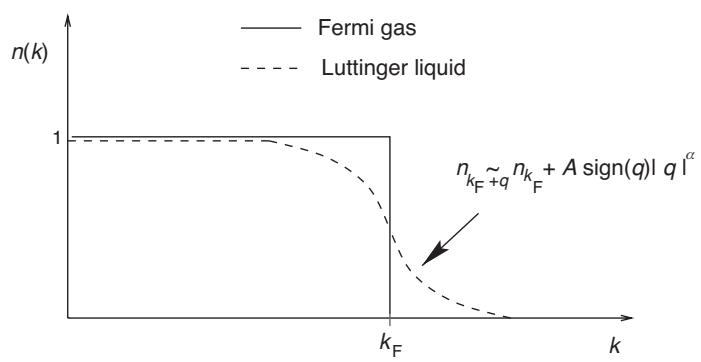
\includegraphics[width=0.62\textwidth]{figs/ch10/fig_10.5_a.jpg}\\[0.8ex]
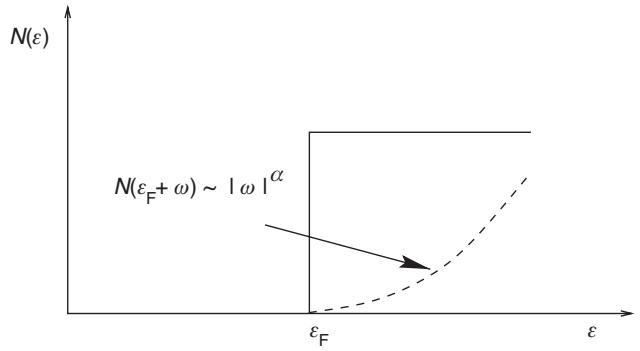
\includegraphics[width=0.60\textwidth]{figs/ch10/fig_10.5_b.jpg}
\caption*{图 10.5\quad 图中给出卢廷格液体（虚线）与费米气体（实线）的动量分布（上图）与隧穿态密度（下图）。图中展示了动量分布函数在费米能量附近的特征性代数依赖。在费米气体极限下，$\alpha=0$，且常数 $A=-1/2$。隧穿态密度在费米能级处消失，正是图 10.6 所示 $I$–$V$ 特性代数式温度依赖的根源。}\label{fig:auto:10.5}
\end{figure}

这样的代数标度预计会产生深刻的实验后果。考虑一个隧穿实验，其中电子越过势垒进入卢廷格液体。通过任何系统的输运都由载流子可资利用的电子态的分布决定。因此可以预期，当 $T\to0$ 时，跨过分隔两个卢廷格液体的势垒的电导（透射率）将趋于零。于是，电导不应以特征激活能的形式随偏离 $T=0$ 而指数式增大，而应以幂律增大（KF1992）。这一幂律应当出现在卢廷格液体输运的电流–电压（$I$–$V$）特性测量中。Chang 及其合作者（CPW1996）在表现出卢廷格液体行为的体系中完成了展示 $I$–$V$ 特性幂律依赖的实验，其数据如图 10.6 所示。在这些特定的实验中，卢廷格液体是分数量子霍尔效应态的边缘态。对于这些样品，Kane 和 Fisher（KF1992）证明电流按如下方式标度：
\begin{equation*}
I\propto T^{\alpha}\left[x+x^{\alpha}\right]
\tag{10.84}
\end{equation*}
其中 $\alpha=3$，$x=eV/2\pi k_{\mathrm{F}}T$。取 $\alpha=2.7$ 以及电压与温度之间的 $1/2\pi$ 标度因子，理论取得了与实验极好的符合。Webb 及其合作者（MUW1996）在量子霍尔体系中，以及 Bockrath 及其同事（B1999）在碳纳米管上也得到了类似结果。由此可见，电子关联是一维电子体系电流–电压特性幂律依赖的核心，这一点已有坚实的实验基础。

\begin{figure}[H]\centering
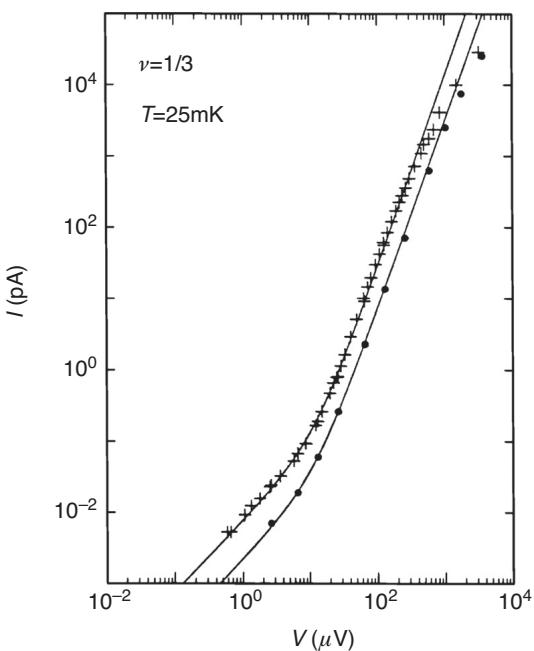
\includegraphics[width=0.48\textwidth]{figs/ch10/fig_10.6.jpg}
\caption*{图 10.6\quad 从体掺杂 $n^{+}$\,GaAs 隧穿进入最低朗道能级填充因子为 $\nu=1/3$ 的分数量子霍尔效应态边缘时的电流–电压（$I$–$V$）特性。实心圆点与十字分别对应磁场 $B=10.8\,\mathrm{T}$ 与 $B=13.4\,\mathrm{T}$。分数量子霍尔态中的边缘态是卢廷格液体。由于隧穿态密度的代数式依赖（见式 (10.82)），隧穿进入卢廷格液体时 $I$ 随 $V$ 预期呈代数式依赖。实曲线是对理论普适形式（式 (10.84)）的拟合。}\label{fig:auto:10.6}
\end{figure}

在本章收尾之际，我们简要评论一下：在半满时保留 Umklapp 项会发生什么。此时电荷部分出现一个余弦项，这意味着在半满时，对排斥相互作用而言电荷部分存在激发能隙。这表明空穴子若不付出巨大的能量代价便不能自由地导电。出现这种情形是因为半满时每个格点上恰好有一个电子，因此把一个电子从一个格点移动到另一个格点的能量代价为 $U$，即电荷能隙的大小。

若 $U$ 为负，则半满时的基态将是每个格点上两个紧紧束缚在一起的电子（结合能量级为 $U$）。这样的实体移动时无需耗费能量。因此，在半满时，只有排斥相互作用才存在电荷能隙。

\section*{小结}
\addcontentsline{toc}{section}{小结}

在一维情形，对存在短程相互作用的电子气，可以发展出一幅关于其集体激发的玻色化图像。这一描述层次使我们能够清晰地证明：一维中自旋与电荷以根本不同的速度运动。至于自旋–电荷分离在 $d>1$ 时如何严格地建立，目前仍属未知。此外，一维中的库仑相互作用导致态密度在费米能级处代数式衰减。态密度的这种特征性衰减是卢廷格液体行为的标志，并且可以在隧穿实验中观测到。某些情形可能需要超出线性近似的物理，那时就必须推广这里介绍的玻色化方法。

\section*{习题}
\addcontentsline{toc}{section}{习题}

\textbf{习题 10.1}\quad 证明：若把式 (10.31) 代入哈密顿量的连续版本（式 (10.6)），所得的玻色哈密顿量将对应于式 (10.30) 的两倍。

\textbf{习题 10.2}\quad 利用式 (10.43) 与 Baker–Hausdorff 恒等式（式 (10.38)）证明
\begin{equation*}
:\mathrm{e}^{\mathcal{A}}::\mathrm{e}^{\mathcal{B}}:=:\mathrm{e}^{\mathcal{A}+\mathcal{B}}:\,\mathrm{e}^{[\mathcal{A}^{-},\mathcal{B}^{+}]}.
\tag{10.85}
\end{equation*}

\textbf{习题 10.3}\quad 证明电流各分量之间的等时对易关系由下式给出：
\begin{equation*}
\left[j_{0}^{\sigma}(x),j_{1}^{\sigma}(y)\right]=-\frac{\mathrm{i}\hbar v_{\mathrm{F}}}{\pi}\partial_{x}\delta(x-y),
\tag{10.86}
\end{equation*}
\begin{equation*}
\left[j_{0}^{\sigma}(x),j_{0}^{\sigma}(y)\right]=\left[j_{1}^{\sigma}(x),j_{1}^{\sigma}(y)\right]=0.
\tag{10.87}
\end{equation*}

\textbf{习题 10.4}\quad 证明式 (10.71) 中的相位因子恒为零。你也许会发现下述攻略有所帮助。首先注意 $\Theta_{\nu}$ 与 $\Phi_{\nu}$ 相对 $g_{\nu}$ 的标度互为倒数，因此各交叉项与重标度因子无关。由连续性方程 $\partial_{\tau}\Phi=\partial_{x}\theta$，你可以确立
\begin{equation*}
\theta(x,\tau)=\int_{-\infty}^{x}\mathrm{d}x'\,\partial_{\tau}\phi(x',\tau)
\tag{10.88}
\end{equation*}
进而确立
\begin{align*}
\langle\tilde{\Phi}_{\nu}(x,\tau)\tilde{\Theta}_{\nu}(0)-\tilde{\Theta}_{\nu}(0)\tilde{\Phi}_{\nu}(0)\rangle&=-\int_{\infty}^{x}\mathrm{d}x'\left\{\partial_{\tau}G(x,x',\tau,0)|_{\tau=0}\right.\\
&\qquad\left.-\partial_{\tau}G(0,x',\tau)|_{x'=0,\tau=0}\right\},
\tag{10.89}
\end{align*}
其中 $G(x,x',\tau,\tau')=\langle\Phi_{\nu}(x,0)\Phi_{\nu}(x',\tau)\rangle$\,\footnote{译注：原书式 (10.89) 的积分下限印作 $\infty$；按式 (10.70) 的定义，此处疑应为 $-\infty$，今照原书排印。}。随后你应能证明余下的贡献以相反的符号进入，因而总和为零。

\textbf{习题 10.5}\quad 计算能级间距为 $\epsilon$ 的无相互作用费米气体的配分函数（取费米海为无限深）。一条求解路径是证明：能量为 $N\epsilon$ 的态，其简并度等于 $N$ 的整数分拆数 $p(N)$（例如 $p(3)=3$，因为 $3=3$、$2+1$、$1+1+1$）。该配分函数对应于什么样的玻色系统？

\textbf{习题 10.6}\quad 推导式 (10.20)。

\section*{参考文献}
\addcontentsline{toc}{section}{参考文献}

\begin{itemize}[leftmargin=2em,itemsep=0pt,parsep=0pt,label={}]
\item [B1999] M. Bockrath, D. H. Cobden, L. Jia, A. G. Rinzler, R. E. Smalley, L. Balents, and P. L. McEuen, \emph{Nature (London)} \textbf{397}, 598 (1999).
\item [BP1953] D. Bohm and D. Pines, \emph{Phys. Rev.} \textbf{92}, 609 (1953).
\item [CPW1996] A. Chang, L. Pfeiffer, and K. West, \emph{Phys. Rev. Lett.} \textbf{77}, 2538 (1996).
\item [H1981] F. D. M. Haldane, \emph{J. Phys. C: Sol. State Phys.} \textbf{14}, 2585 (1981).
\item [H1964] J. Hubbard, \emph{Proc. Roy. Soc. A} \textbf{277}, 237 and 281 (1964).
\item [KF1992] C. L. Kane and M. P. A. Fisher, \emph{Phys. Rev. Lett.} \textbf{68}, 1220 (1992).
\item [KS1996] G. Kotliar and Q. Si, \emph{Phys. Rev. B} \textbf{53} (1996).
\item [L1960] J. M. Luttinger, \emph{Phys. Rev.} \textbf{119}, 1153 (1960).
\item [M1975] S. Mandelstam, \emph{Phys. Rev. D} \textbf{11}, 3026 (1975).
\item [M1974] D. Mattis, \emph{J. Math. Phys. (N.Y.)} \textbf{15}, 609 (1974).
\item [ML1965] D. Mattis and E. Lieb, \emph{J. Math. Phys.} \textbf{6}, 304 (1965).
\item [MUW1996] F. P. Milliken, C. P. Umbach, and R. A. Webb, \emph{Solid State Commun.} \textbf{97}, 309 (1996).
\item [S1990] H. J. Schulz, \emph{Phys. Rev. Lett.} \textbf{64}, 2831 (1990).
\item [S1959] J. Schwinger, \emph{Phys. Rev. Lett.} \textbf{3}, 296 (1959).
\item [T1950] S. Tomonaga, \emph{Prog. Theor. Phys. (Kyoto)} \textbf{5}, 544 (1950).
\item [VDS1998] J. von Delft and H. Schoeller, \emph{Annalen Phys.} \textbf{7}, 225 (1998).
\item [Y2005] A. Yacoby, \emph{Les Houches Summer School Proceedings} \textbf{81}, 605 (2005).
\end{itemize}
